%!TeX encoding = UTF-8
%!TeX program = xelatex
\documentclass[notheorems, aspectratio=54]{beamer}
% aspectratio: 1610, 149, 54, 43(default), 32

\usepackage{latexsym}
\usepackage{amsmath,amssymb}
\usepackage{mathtools}
\usepackage{color,xcolor}
\usepackage{graphicx}
\usepackage{algorithm}
\usepackage{amsthm}
\usepackage{lmodern} % 解决 font warning
% \usepackage[UTF8]{ctex}
\usepackage{animate} % insert gif

\usepackage{lipsum} % To generate test text 
\usepackage{ulem} % 下划线,波浪线

\usepackage{listings} % display code on slides; don't forget [fragile] option after \begin{frame}

% ----------------------------------------------
% tikx
\usepackage{framed}
\usepackage{tikz}
\usepackage{pgf}
\usetikzlibrary{calc,trees,positioning,arrows,chains,shapes.geometric,%
    decorations.pathreplacing,decorations.pathmorphing,shapes,%
    matrix,shapes.symbols}
\pgfmathsetseed{1} % To have predictable results
% Define a background layer, in which the parchment shape is drawn
\pgfdeclarelayer{background}
\pgfsetlayers{background,main}

% define styles for the normal border and the torn border
\tikzset{
  normal border/.style={orange!30!black!10, decorate, 
     decoration={random steps, segment length=2.5cm, amplitude=.7mm}},
  torn border/.style={orange!30!black!5, decorate, 
     decoration={random steps, segment length=.5cm, amplitude=1.7mm}}}

% Macro to draw the shape behind the text, when it fits completly in the
% page
\def\parchmentframe#1{
\tikz{
  \node[inner sep=2em] (A) {#1};  % Draw the text of the node
  \begin{pgfonlayer}{background}  % Draw the shape behind
  \fill[normal border] 
        (A.south east) -- (A.south west) -- 
        (A.north west) -- (A.north east) -- cycle;
  \end{pgfonlayer}}}

% Macro to draw the shape, when the text will continue in next page
\def\parchmentframetop#1{
\tikz{
  \node[inner sep=2em] (A) {#1};    % Draw the text of the node
  \begin{pgfonlayer}{background}    
  \fill[normal border]              % Draw the ``complete shape'' behind
        (A.south east) -- (A.south west) -- 
        (A.north west) -- (A.north east) -- cycle;
  \fill[torn border]                % Add the torn lower border
        ($(A.south east)-(0,.2)$) -- ($(A.south west)-(0,.2)$) -- 
        ($(A.south west)+(0,.2)$) -- ($(A.south east)+(0,.2)$) -- cycle;
  \end{pgfonlayer}}}

% Macro to draw the shape, when the text continues from previous page
\def\parchmentframebottom#1{
\tikz{
  \node[inner sep=2em] (A) {#1};   % Draw the text of the node
  \begin{pgfonlayer}{background}   
  \fill[normal border]             % Draw the ``complete shape'' behind
        (A.south east) -- (A.south west) -- 
        (A.north west) -- (A.north east) -- cycle;
  \fill[torn border]               % Add the torn upper border
        ($(A.north east)-(0,.2)$) -- ($(A.north west)-(0,.2)$) -- 
        ($(A.north west)+(0,.2)$) -- ($(A.north east)+(0,.2)$) -- cycle;
  \end{pgfonlayer}}}

% Macro to draw the shape, when both the text continues from previous page
% and it will continue in next page
\def\parchmentframemiddle#1{
\tikz{
  \node[inner sep=2em] (A) {#1};   % Draw the text of the node
  \begin{pgfonlayer}{background}   
  \fill[normal border]             % Draw the ``complete shape'' behind
        (A.south east) -- (A.south west) -- 
        (A.north west) -- (A.north east) -- cycle;
  \fill[torn border]               % Add the torn lower border
        ($(A.south east)-(0,.2)$) -- ($(A.south west)-(0,.2)$) -- 
        ($(A.south west)+(0,.2)$) -- ($(A.south east)+(0,.2)$) -- cycle;
  \fill[torn border]               % Add the torn upper border
        ($(A.north east)-(0,.2)$) -- ($(A.north west)-(0,.2)$) -- 
        ($(A.north west)+(0,.2)$) -- ($(A.north east)+(0,.2)$) -- cycle;
  \end{pgfonlayer}}}

% Define the environment which puts the frame
% In this case, the environment also accepts an argument with an optional
% title (which defaults to ``Example'', which is typeset in a box overlaid
% on the top border
\newenvironment{parchment}[1][Example]{%
  \def\FrameCommand{\parchmentframe}%
  \def\FirstFrameCommand{\parchmentframetop}%
  \def\LastFrameCommand{\parchmentframebottom}%
  \def\MidFrameCommand{\parchmentframemiddle}%
  \vskip\baselineskip
  \MakeFramed {\FrameRestore}
  \noindent\tikz\node[inner sep=1ex, draw=black!20,fill=white, 
          anchor=west, overlay] at (0em, 2em) {\sffamily#1};\par}%
{\endMakeFramed}

% ----------------------------------------------

\mode<presentation>{
    \usetheme{CambridgeUS}
    % Boadilla CambridgeUS
    % default Antibes Berlin Copenhagen
    % Madrid Montpelier Ilmenau Malmoe
    % Berkeley Singapore Warsaw
    \usecolortheme{beaver}
    % beetle, beaver, orchid, whale, dolphin
    \useoutertheme{infolines}
    % infolines miniframes shadow sidebar smoothbars smoothtree split tree
    \useinnertheme{circles}
    % circles, rectanges, rounded, inmargin
}
% 设置 block 颜色
\setbeamercolor{block title}{bg=red!30,fg=white}

\newcommand{\reditem}[1]{\setbeamercolor{item}{fg=red}\item #1}

% 缩放公式大小
\newcommand*{\Scale}[2][4]{\scalebox{#1}{\ensuremath{#2}}}

% 解决 font warning
\renewcommand\textbullet{\ensuremath{\bullet}}

% ---------------------------------------------------------------------
% flow chart
\tikzset{
    >=stealth',
    punktchain/.style={
        rectangle, 
        rounded corners, 
        % fill=black!10,
        draw=white, very thick,
        text width=6em,
        minimum height=2em, 
        text centered, 
        on chain
    },
    largepunktchain/.style={
        rectangle,
        rounded corners,
        draw=white, very thick,
        text width=10em,
        minimum height=2em,
        on chain
    },
    line/.style={draw, thick, <-},
    element/.style={
        tape,
        top color=white,
        bottom color=blue!50!black!60!,
        minimum width=6em,
        draw=blue!40!black!90, very thick,
        text width=6em, 
        minimum height=2em, 
        text centered, 
        on chain
    },
    every join/.style={->, thick,shorten >=1pt},
    decoration={brace},
    tuborg/.style={decorate},
    tubnode/.style={midway, right=2pt},
    font={\fontsize{10pt}{12}\selectfont},
}
% ---------------------------------------------------------------------

% code setting
\lstset{
    language=C++,
    basicstyle=\ttfamily\footnotesize,
    keywordstyle=\color{red},
    breaklines=true,
    xleftmargin=2em,
    numbers=left,
    numberstyle=\color[RGB]{222,155,81},
    frame=leftline,
    tabsize=4,
    breakatwhitespace=false,
    showspaces=false,               
    showstringspaces=false,
    showtabs=false,
    morekeywords={Str, Num, List},
}

% ---------------------------------------------------------------------

%% preamble
\title[Data Management in Deep Learning Task]{Data Management in Deep Learning Task}
% \subtitle{The subtitle}
\author{Xie Jian}
\institute[]{I2EC, ICS, NJU}

% -------------------------------------------------------------

\begin{document}

%% title frame
\begin{frame}
    \titlepage
\end{frame}

%% normal frame

% table of content
\begin{frame}
    \frametitle{Table of Contents}
    \tableofcontents
\end{frame}
\AtBeginSection[]
{
    \begin{frame}
        \frametitle{Table of Contents}
        \tableofcontents[currentsection]
    \end{frame}
}
% -----------------------------------------------

\section{Introduction}
\begin{frame}
    \frametitle{Pipeline}
    \centering
    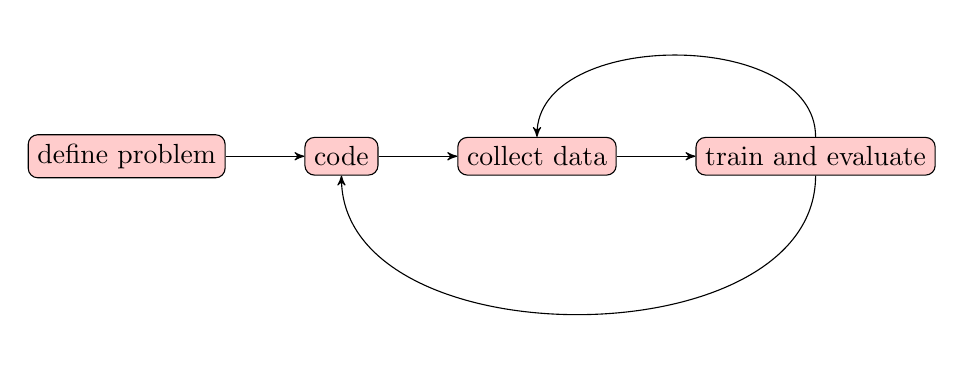
\begin{tikzpicture}
    [
        level distance=4cm,
        level 1/.style={sibling distance=5cm},
        level 2/.style={sibling distance=2.5cm},
        level 3/.style={sibling distance=1cm},
        every node/.style={shape=rectangle, rounded corners=.8ex, draw, fill = red!20},
        bigbox/.style={shape=rectangle, rounded corners=.8ex, draw, fill=blue!20, minimum, height=3cm, minimum width=9cm},
    ]
    
    \node(task){define problem};
    \node(code)[right=of task]{code};
    \node(col) [right=of code]{collect data};
    \node(test) [right=of col]{train and evaluate};
    \draw[->] (task) to (code);
    \draw[->] (code) to (col);
    \draw[->] (col) to (test);
    \draw[->] (test) to[out=90,in=90] (col);
    \draw[->] (test) to[out=-90,in=-90] (code);
    \end{tikzpicture}
\end{frame}
\begin{frame}
    \frametitle{Structure}
    \centering
    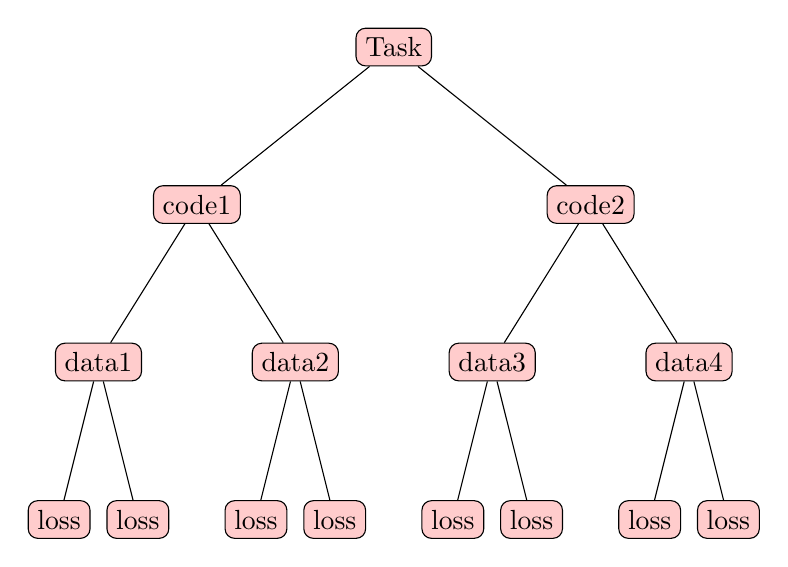
\begin{tikzpicture}
[
    level distance=2cm,
    level 1/.style={sibling distance=5cm},
    level 2/.style={sibling distance=2.5cm},
    level 3/.style={sibling distance=1cm},
    first/.style={level distance=6ex},
    second/.style={level distance=12ex},
    third/.style={level distance=18ex},
    common/.style={shape = rectangle, rounded corners=.8ex, draw, fill = red!20},
    highlight/.style={shape=rectangle, rounded corners=.8ex, draw, fill = red!50},
]
\node[common] {Task}
    child {node[common]{code1}
        child {node[common]{data1}
            child {node[common]{loss}}
            child {node[common]{loss}}
        }
        child {node[common]{data2}
            child {node[common]{loss}}
            child {node[common]{loss}}
        }
    }
    child {node[common]{code2}
        child {node[common]{data3}
            child {node[common]{loss}}
            child {node[common]{loss}}
        }
        child {node[common]{data4}
            child {node[common]{loss}}
            child {node[common]{loss}}
        }
    };
\end{tikzpicture}
\end{frame}

\begin{frame}
    \frametitle{Code Management}
    \centering
    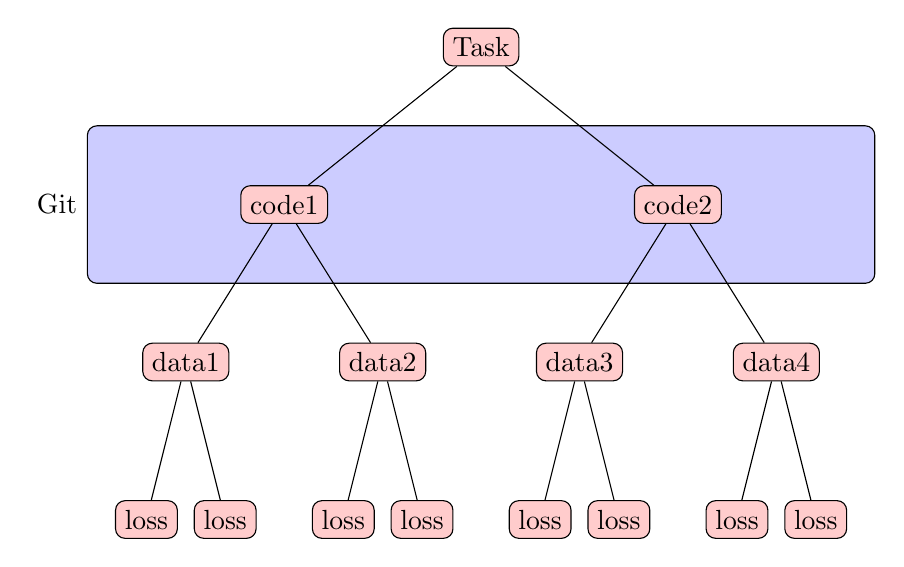
\begin{tikzpicture}
[
    level distance=2cm,
    level 1/.style={sibling distance=5cm},
    level 2/.style={sibling distance=2.5cm},
    level 3/.style={sibling distance=1cm},
    first/.style={level distance=6ex},
    second/.style={level distance=12ex},
    third/.style={level distance=18ex},
    common/.style={shape=rectangle, rounded corners=.8ex, draw, fill = red!20},
    highlight/.style={shape=rectangle, rounded corners=.8ex, draw, fill = red!50},
    bigbox/.style={shape=rectangle, rounded corners=.8ex, draw, fill=blue!20, minimum height=2cm, minimum width=10cm},
]
\node at (0, -2) [bigbox, label=west:Git]{};
\node[common] {Task}
    child {node(code1)[common]{code1}
        child {node[common]{data1}
            child {node[common]{loss}}
            child {node[common]{loss}}
        }
        child {node(code2)[common]{data2}
            child {node[common]{loss}}
            child {node[common]{loss}}
        }
    }
    child {node[common]{code2}
        child {node[common]{data3}
            child {node[common]{loss}}
            child {node[common]{loss}}
        }
        child {node[common]{data4}
            child {node[common]{loss}}
            child {node[common]{loss}}
        }
    };
\end{tikzpicture}
\end{frame}
\begin{frame}
    \frametitle{Others Management}
    \centering
    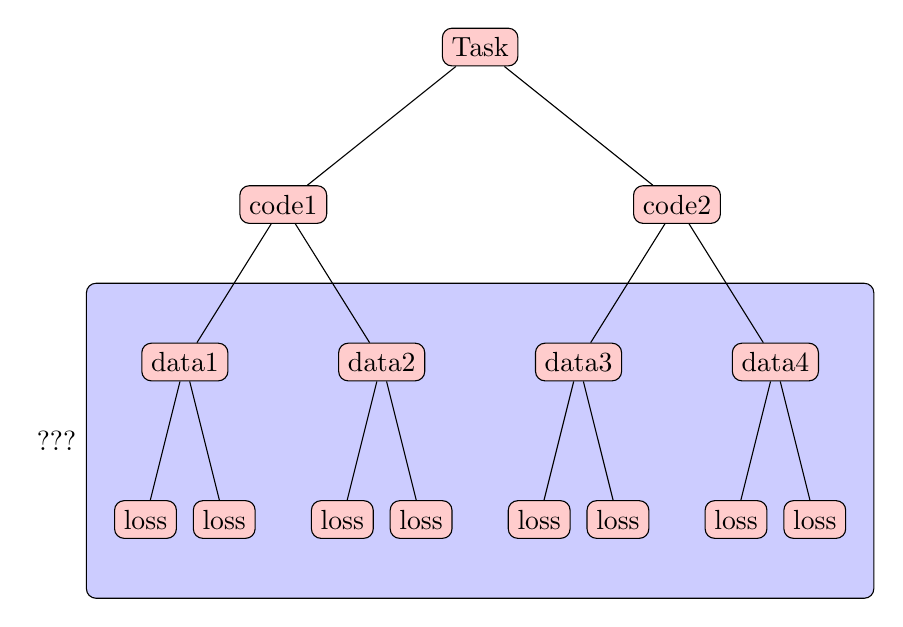
\begin{tikzpicture}
[
    level distance=2cm,
    level 1/.style={sibling distance=5cm},
    level 2/.style={sibling distance=2.5cm},
    level 3/.style={sibling distance=1cm},
    first/.style={level distance=6ex},
    second/.style={level distance=12ex},
    third/.style={level distance=18ex},
    common/.style={shape=rectangle, rounded corners=.8ex, draw, fill = red!20},
    highlight/.style={shape=rectangle, rounded corners=.8ex, draw, fill = red!50},
    bigbox/.style={shape=rectangle, rounded corners=.8ex, draw, fill=blue!20, minimum height=4cm, minimum width=10cm},
]
\node at (0, -5) [bigbox, label=west:???]{};
\node[common] {Task}
    child {node(code1)[common]{code1}
        child {node[common]{data1}
            child {node[common]{loss}}
            child {node[common]{loss}}
        }
        child {node(code2)[common]{data2}
            child {node[common]{loss}}
            child {node[common]{loss}}
        }
    }
    child {node[common]{code2}
        child {node[common]{data3}
            child {node[common]{loss}}
            child {node[common]{loss}}
        }
        child {node[common]{data4}
            child {node[common]{loss}}
            child {node[common]{loss}}
        }
    };
\end{tikzpicture}
\end{frame}

\begin{frame}
    \frametitle{Why need it}
    Model = Algorithm + Data
    \begin{block}{Problem}
        For image classification tasks, the model has a bad performance in night
    \end{block} \pause
    \begin{block}{Solution}
        Train with more night images\\
        Try new network and new loss function
    \end{block} \pause
    \begin{block}{Management}
        Datasets with different number of night images\\
        Loss associate with different Datasets \\
        Loss associate with different net
    \end{block}
\end{frame}

\section{Implementation}
\begin{frame}[fragile]
\frametitle{Shema}
\begin{lstlisting}
    {
        //data content
        "data":{
            "name": "xxx" //data name
            "data": "xxx"  //data content / data url
        },
        //data label
        label:{
            "label1":xxx,
            "label2":xxx
        },
        //data categories
        categories:{
            "cate1":"xxx",
            "cate2":"xxx"
        }
    }
\end{lstlisting}
\end{frame}

\begin{frame}
    \frametitle{Architecture}
    \centering
    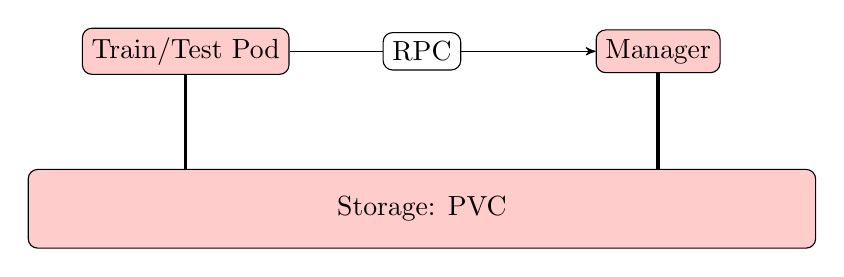
\begin{tikzpicture}
[
    level distance=4cm,
    level 1/.style={sibling distance=5cm},
    level 2/.style={sibling distance=2.5cm},
    level 3/.style={sibling distance=1cm},
    every node/.style={shape=rectangle, rounded corners=.8ex, draw, fill = red!20},
]
\node(GPU) at (-3, 0){Train/Test Pod};
\node(Ma) at (3, 0){Manager};
\node(PVC) at (0, -2)[minimum width = 10cm, minimum height = 1cm]{Storage: PVC};
\draw[->] (GPU) to (Ma); 
\node[fill=white]{RPC};
\draw[-, very thick ] (GPU) to (-3, -1.5);
\draw[-, very thick ] (3,-0.28) to (3, -1.5);
\end{tikzpicture}
\end{frame}

\begin{frame}
    \frametitle{QueryData}
    \centering
    "name": RL,\\
    "cate": RL ....
    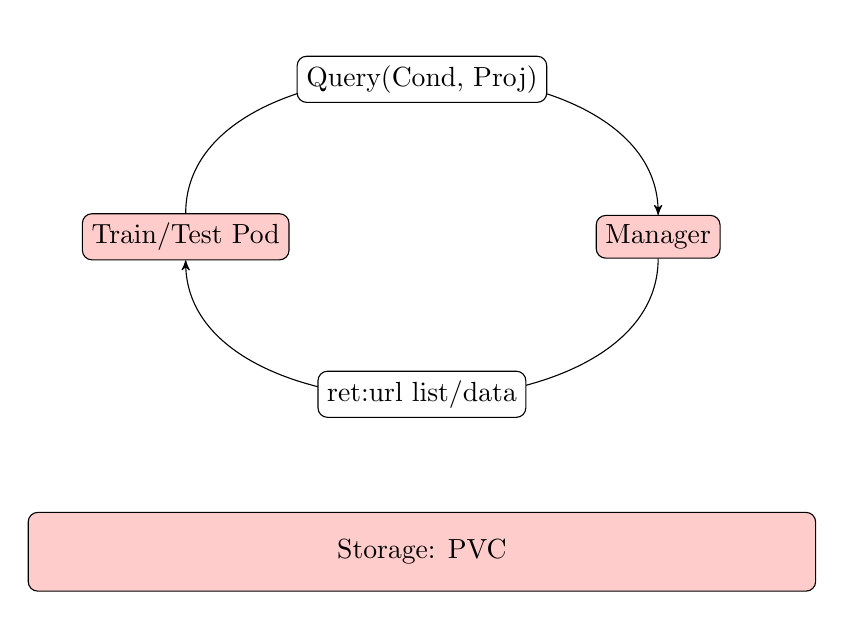
\begin{tikzpicture}
[
    level distance=4cm,
    level 1/.style={sibling distance=5cm},
    level 2/.style={sibling distance=2.5cm},
    level 3/.style={sibling distance=1cm},
    every node/.style={shape=rectangle, rounded corners=.8ex, draw, fill = red!20},
]
\node(GPU) at (-3, 2){Train/Test Pod};
\node(Ma) at (3, 2){Manager};
\node(PVC) at (0, -2)[minimum width = 10cm, minimum height = 1cm]{Storage: PVC};
\draw[->] (GPU) to[in=90,out=90] (Ma);
\node at (0,4)[fill=white]{Query(Cond, Proj)};
\draw[->] (Ma) to[in=-90,out=-90] (GPU);
\node[fill=white]{ret:url list/data};
\end{tikzpicture}
\end{frame}

\begin{frame}
    \frametitle{SkipList}
    \centering
    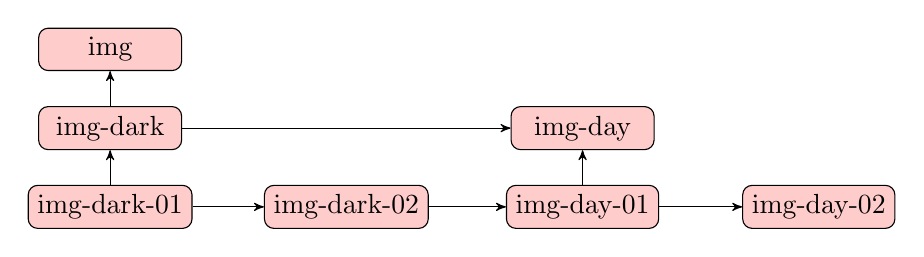
\begin{tikzpicture}
[
    level distance=4cm,
    level 1/.style={sibling distance=5cm},
    level 2/.style={sibling distance=2.5cm},
    level 3/.style={sibling distance=1cm},
    every node/.style={shape=rectangle, rounded corners=.8ex, draw, fill = red!20},
    bigbox/.style={shape=rectangle, rounded corners=.8ex, draw, fill=blue!20, minimum, height=3cm, minimum width=9cm},
]

\node(ik1) at (-4.5,-1){img-dark-01};
\node(ik2) at (-1.5,-1) []{img-dark-02};
\node(id1) at (1.5,-1) []{img-day-01};
\node(id2) at (4.5,-1) []{img-day-02};
\draw[->] (ik1) to (ik2);
\draw[->] (ik2) to (id1);
\draw[->] (id1) to (id2);

\node(ik) at (-4.5,0)[minimum width=12ex]{img-dark};
\node(id) at (1.5,0) [minimum width=12ex]{img-day};
\draw[->] (ik) to (id);

\node(i) at (-4.5,1)[minimum width=12ex]{img};

\draw[->] (ik) to (i);
\draw[->] (ik1) to (ik);
\draw[->] (id1) to (id);

\end{tikzpicture}
\end{frame}

\begin{frame}
    \frametitle{LoadData}
    \centering
    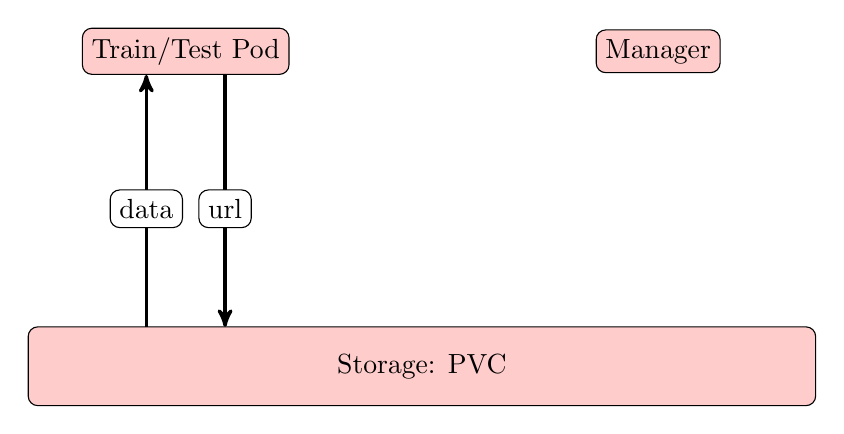
\begin{tikzpicture}
[
    level distance=4cm,
    level 1/.style={sibling distance=5cm},
    level 2/.style={sibling distance=2.5cm},
    level 3/.style={sibling distance=1cm},
    every node/.style={shape=rectangle, rounded corners=.8ex, draw, fill = red!20},
]
\node(GPU) at (-3, 2){Train/Test Pod};
\node(Ma) at (3, 2){Manager};
\node(PVC) at (0, -2)[minimum width = 10cm, minimum height = 1cm]{Storage: PVC};
\draw[->, very thick] (-2.5, 1.7) to (-2.5, -1.5);
\node at (-2.5, 0)[fill=white]{url};
\draw[->, very thick] (-3.5, -1.5) to (-3.5, 1.7);
\node at (-3.5,0)[fill=white]{data};
\end{tikzpicture}
\end{frame}

\section{Next Step}

\begin{frame}
    \frametitle{with Git}
    \centering
    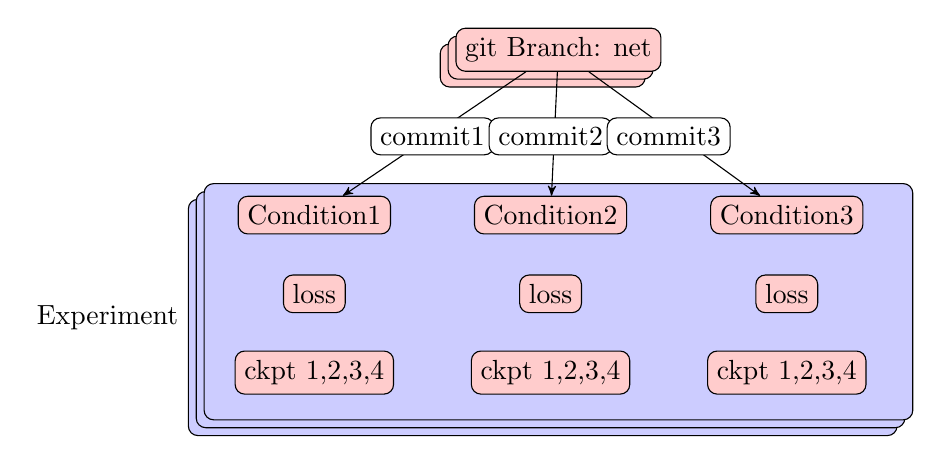
\begin{tikzpicture}
[
    level distance=4cm,
    level 1/.style={sibling distance=5cm},
    level 2/.style={sibling distance=2.5cm},
    level 3/.style={sibling distance=1cm},
    every node/.style={shape=rectangle, rounded corners=.8ex, draw, fill = red!20},
    bigbox/.style={shape=rectangle, rounded corners=.8ex, draw, fill=blue!20, minimum height=3cm, minimum width=9cm},
]
\node at (-0.1, 2.9){git Branch: net};
\node at (0,3.0){git Branch: net};
\node(branch) at (0.1, 3.1){git Branch: net};
\node at (-0.1,-0.3) [fill=blue!20, bigbox, label=west:Experiment] {};
\node at (0,-0.2) [fill=blue!20, bigbox] {};
\node at (0.1,-0.1) [fill=blue!20, bigbox] {};
\node(cond1) at (-3,1){Condition1};
\node(cond2) at (0,1){Condition2};
\node(cond3) at (3,1){Condition3};
\node(loss) at (0,0){loss};
\node(ckpt) at (0,-1){ckpt 1,2,3,4};
\node(loss) at (-3,0){loss};
\node(ckpt) at (-3,-1){ckpt 1,2,3,4};
\node(loss) at (3,0){loss};
\node(ckpt) at (3,-1){ckpt 1,2,3,4};
\draw[->] (branch) to (cond1);
\node at (-1.5, 2)[fill=white]{commit1};
\draw[->] (branch) to (cond2);
\node at (0, 2)[fill=white]{commit2};
\draw[->] (branch) to (cond3);
\node at (1.5, 2)[fill=white]{commit3};
\end{tikzpicture}
\end{frame}

\begin{frame}
    \frametitle{with Git}
    \begin{itemize}
    \item Associate Experiment with branch
    \item Associate Datasets/Condition with commit
    \end{itemize}
\end{frame}
\end{document}